% CEFN_v2_architecture.tex
% Compact publication-ready architecture diagram for CEFN v2
% Compile with: pdflatex CEFN_v2_architecture.tex
\documentclass[tikz,border=5pt]{standalone}
\usepackage{tikz}
\usepackage{amsmath,amssymb}
\usetikzlibrary{positioning,fit,backgrounds,arrows.meta,calc,shapes.geometric}

% Color palette (consistent with paper figures)
\definecolor{cefnblue}{HTML}{2E86AB}
\definecolor{evo2mag}{HTML}{A23B72}
\definecolor{amorange}{HTML}{F18F01}
\definecolor{dstred}{HTML}{C73E1D}
\definecolor{gray}{HTML}{8D99AE}
\definecolor{dark}{HTML}{2B2D42}
\definecolor{lightbg}{HTML}{EDF2F4}
\definecolor{nodefill}{HTML}{F8F9FA}

\begin{document}
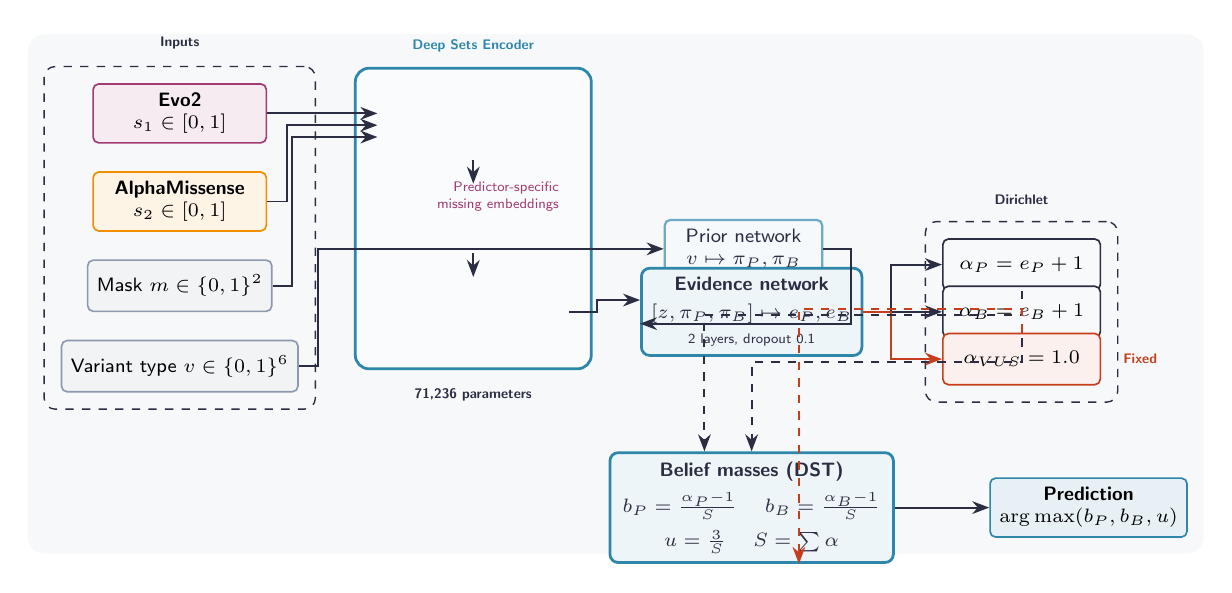
\begin{tikzpicture}[
    font=\sffamily\footnotesize,
    >=Stealth,
    thick,
    % Node styles
    input/.style={rectangle, rounded corners=2pt, draw=dark, fill=nodefill,
                  minimum width=2.2cm, minimum height=0.65cm, align=center,
                  line width=0.6pt, font=\sffamily\scriptsize},
    block/.style={rectangle, rounded corners=3pt, draw=cefnblue, fill=cefnblue!8,
                  minimum width=2.4cm, minimum height=0.85cm, align=center,
                  line width=1pt, text=dark, font=\sffamily\scriptsize},
    smallblock/.style={rectangle, rounded corners=2pt, draw=cefnblue!70, fill=cefnblue!5,
                       minimum width=2.0cm, minimum height=0.65cm, align=center,
                       line width=0.8pt, text=dark, font=\sffamily\scriptsize},
    output/.style={rectangle, rounded corners=2pt, draw=dark, fill=nodefill,
                   minimum width=2.0cm, minimum height=0.65cm, align=center,
                   line width=0.6pt, font=\sffamily\scriptsize},
    arrow/.style={->, line width=0.7pt, draw=dark},
    label/.style={font=\sffamily\tiny, text=gray},
]

% =============================================================================
% COLUMN 1: INPUTS (stacked vertically)
% =============================================================================
\node[input, fill=evo2mag!10, draw=evo2mag] (evo2) 
    {\textbf{Evo2}\\$s_1 \in [0,1]$};
\node[input, fill=amorange!10, draw=amorange, below=0.35cm of evo2] (am) 
    {\textbf{AlphaMissense}\\$s_2 \in [0,1]$};
\node[input, fill=gray!12, draw=gray, below=0.35cm of am] (mask) 
    {Mask $m \in \{0,1\}^2$};
\node[input, fill=gray!12, draw=gray, below=0.35cm of mask] (vartype) 
    {Variant type $v \in \{0,1\}^6$};

\node[fit=(evo2)(vartype), inner sep=6pt, rounded corners=4pt, 
      draw=dark, line width=0.5pt, dashed] (inputbox) {};
\node[label, above=0.08cm of inputbox.north, text=dark] {\textbf{Inputs}};

% =============================================================================
% COLUMN 2: DEEP SETS ENCODER (vertical stack)
% =============================================================================
\node[block, right=1.4cm of evo2, yshift=-0.15cm] (phi) 
    {Element-wise $\phi$\\$[s_i, m_i, e_i] \mapsto h_i$};
\node[block, below=0.3cm of phi] (pool) 
    {Mean pool\\$z = \frac{1}{n}\sum_i h_i$};
\node[block, below=0.3cm of pool] (rho) 
    {Aggregation $\rho$\\$z \in \mathbb{R}^{128}$};

\node[fit=(phi)(rho), inner sep=8pt, rounded corners=5pt,
      draw=cefnblue, line width=1pt, fill=cefnblue!3] (deepsetbox) {};
\node[label, above=0.06cm of deepsetbox.north, text=cefnblue] 
    {\textbf{Deep Sets Encoder}};

% Missing embedding note
\node[label, below=0.15cm of phi.south east, anchor=north east, text=evo2mag, align=right] 
    {Predictor-specific\\missing embeddings};

% =============================================================================
% COLUMN 3: PRIOR + EVIDENCE (side by side)
% =============================================================================
\node[smallblock, right=1.2cm of rho, yshift=0.8cm] (prior) 
    {Prior network\\$v \mapsto \pi_P, \pi_B$};
\node[label, below=0.05cm of prior.south, text=cefnblue!70] {Variant-type conditioned};

\node[block, right=0.9cm of rho, minimum width=2.8cm, minimum height=1.0cm] (evidence) 
    {\textbf{Evidence network}\\[2pt]
     $[z, \pi_P, \pi_B] \mapsto e_P, e_B$\\[1pt]
     \tiny 2 layers, dropout 0.1};

% =============================================================================
% COLUMN 4: DIRICHLET OUTPUTS
% =============================================================================
\node[output, right=1.0cm of evidence, yshift=0.6cm] (alphaP) 
    {$\alpha_P = e_P + 1$};
\node[output, right=1.0cm of evidence, yshift=0cm] (alphaB) 
    {$\alpha_B = e_B + 1$};
\node[output, fill=dstred!8, draw=dstred, right=1.0cm of evidence, yshift=-0.6cm] (alphaV) 
    {$\alpha_{VUS} = 1.0$};

\node[fit=(alphaP)(alphaV), inner sep=6pt, rounded corners=4pt,
      draw=dark, line width=0.5pt, dashed] (outputbox) {};
\node[label, above=0.08cm of outputbox.north, text=dark] {\textbf{Dirichlet}};

% VUS annotation
\node[label, right=0.15cm of alphaV.east, text=dstred, align=left] 
    {\textbf{Fixed}};

% =============================================================================
% COLUMN 5: BELIEF + PREDICTION (below, connected)
% =============================================================================
\node[block, below=1.2cm of evidence, minimum width=3.6cm, minimum height=1.1cm] (belief) 
    {\textbf{Belief masses (DST)}\\[3pt]
     $b_P = \frac{\alpha_P - 1}{S}$ \quad
     $b_B = \frac{\alpha_B - 1}{S}$\\[3pt]
     $u = \frac{3}{S}$ \quad
     $S = \sum \alpha$};

\node[output, fill=cefnblue!12, draw=cefnblue, right=1.2cm of belief] (pred) 
    {\textbf{Prediction}\\$\arg\max(b_P, b_B, u)$};

% =============================================================================
% ARROWS
% =============================================================================
% Inputs to phi
\draw[arrow] (evo2.east) -- ++(0.25,0) |- ([yshift=0.15cm]phi.west);
\draw[arrow] (am.east) -- ++(0.25,0) |- (phi.west);
\draw[arrow] (mask.east) -- ++(0.25,0) |- ([yshift=-0.15cm]phi.west);

% Phi -> pool -> rho
\draw[arrow] (phi) -- (pool);
\draw[arrow] (pool) -- (rho);

% Vartype to prior
\draw[arrow] (vartype.east) -- ++(0.25,0) |- (prior.west);

% Rho and prior to evidence
\draw[arrow] (rho.east) -- ++(0.35,0) |- ([yshift=0.15cm]evidence.west);
\draw[arrow] (prior.east) -- ++(0.35,0) |- ([yshift=-0.15cm]evidence.west);

% Evidence to alphas
\draw[arrow] (evidence.east) -- ++(0.35,0) |- (alphaP.west);
\draw[arrow] (evidence.east) -- ++(0.35,0) |- (alphaB.west);
\draw[arrow, draw=dstred] (evidence.east) -- ++(0.35,0) |- (alphaV.west);

% Alphas to belief (dashed, curved)
\draw[arrow, dashed] (alphaP.south) -- ++(0,-0.3) -| ([xshift=-0.6cm]belief.north);
\draw[arrow, dashed] (alphaB.south) -- ++(0,-0.3) -| (belief.north);
\draw[arrow, dashed, draw=dstred] (alphaV.north) -- ++(0,0.3) -| ([xshift=0.6cm]belief.south);

% Belief to prediction
\draw[arrow] (belief) -- (pred);

% =============================================================================
% PARAMETER COUNT
% =============================================================================
\node[label, below=0.1cm of deepsetbox.south, text=dark] 
    {\textbf{71,236 parameters}};

% =============================================================================
% BACKGROUND
% =============================================================================
\begin{scope}[on background layer]
    \fill[lightbg, rounded corners=6pt, opacity=0.5]
        ($(inputbox.north west)+(-0.2,0.4)$) rectangle
        ($(pred.south east)+(0.2,-0.2)$);
\end{scope}

\end{tikzpicture}
\end{document}
